\section{Methodology and Data}


Als Daten wurden die Bundestagsprotokolle im Zeitraum von 2009 bis 2018 vom Archiv der Bundestagswebsite\thanks {https://www.bundestag.de/service/opendatav} heruntergeladen und in einen R-Datensatz eingelesen. Dabei haben sich die XML-Files vor 2017 von den XML-Files nach 2017 dahingehend unterschieden, dass die Plenarprotokolle vor 2017 nicht in XML-Nodes aufgegliedert waren. Daher wurden zwei unterschiedliche R-Skripte verwendet: Die Daten nach 2017 wurde mit xPath in den R-Datensatz eingelesen und die Daten von vor 2017 mit regulären Ausdrücken. Dafür wurde auch die Stammdatendatei der Politiker verwendet, die aus dem selben Archiv stammt, um die Namen der Politiker als Redner in den entsprechenden Legislaturperioden identifizieren zu können. Dadurch erst konnten die Plenarprotokolle in einzelne Bundestagsreden aufgeschlüsselt werden. Der Beginn einer Rede lässt sich durch den Namen von einem Politiker gefolgt von seiner Partei in Klammern und einem Doppelpunkt, oder der Name von einem Politiker gefolgt von einem Doppelpunkt, wenn dieser keiner Partei angehört identifizieren. Als Beispiel: 
\begin{verbatim}
str_split(text, paste0(c("(?<=.)(?=(",namenregex,")(?=(:| (\\(.{1,40}\\):))))")
\end{verbatim}
Der daraus entstehende Datensatz umfasst \verb 48.919  Reden im Zeitraum von 2009 bis 2017 und 13 Variablen. In einer Zeile steht eine Aktion, die eindeutig einer Partei zugeordent werden kann.\\

\noindent 
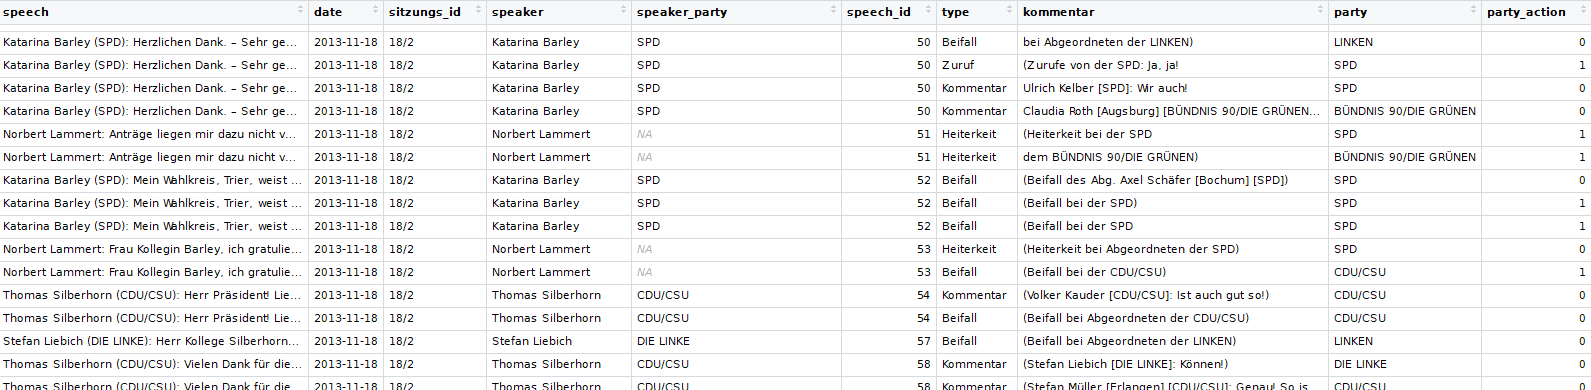
\includegraphics[width=\linewidth]{Grafiken/Head_Reden.PNG}
\\

 



